\textbf{ID:} UC07 (View Event) \\
\textbf{Scope:} CS Automated Information Timeline \\
\textbf{Level:} User Goal \\
\textbf{Primary Actor:} Faculty \\
\textbf{Stakeholders and Interests:}
\begin{itemize}
    \item Audience: Wants to view up-to-date information about events in the CS Department
    \item Faculty: Wants the ability to view events they have submitted
    \item Office Manager: Wants to display calendar events on the Lobby TV
    \item Admin/Reviewer: Wants to view events submitted by Faculty so they can review them
\end{itemize}
\textbf{Preconditions:} Faculty created an event (UC04) and submitted it for review (UC08). Admin/Reviewer reviewed the event (UC09) and approved. Faculty is identified and authenticated in the system and is viewing the event calendar (UC03). \\
\textbf{Postconditions:} Event status is in an approved state. \\
\textbf{Main Success Scenario:}
\begin{enumerate}
    \item Faculty clicks the “View My Events” link on the event calendar page.
    \item System returns a list of existing events authored by Faculty that have been approved.
    \item Faculty selects the event they wish to view from the returned list of their previously approved events.
    \item System returns the event page for the selected event.
\end{enumerate}
\textbf{Extensions (or Alternate Flows):} \\
3a. Faculty does not see the event they wish to view in the returned list because the event has not yet been approved by the Admin/Reviewer:
\begin{enumerate}
    \item Faculty must wait for approval from Admin/Reviewer on the original event before the event is eligible for viewing from the event calendar.
\end{enumerate}
\textbf{Special Requirements:} None \\
\textbf{Technology and Data Variations List:} None \\
\textbf{Frequency of Occurrence:} Continuous \\
\textbf{Open Issues:} None \\

\begin{figure}[H]
    \centering
    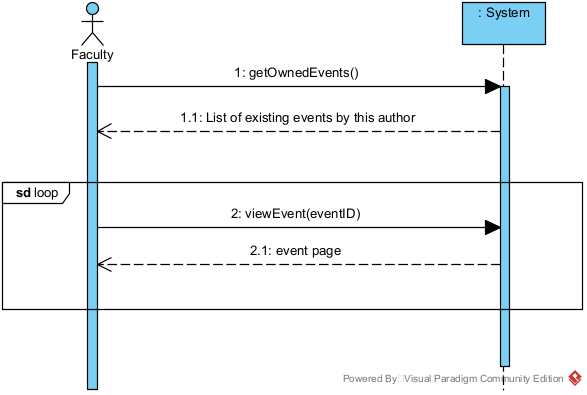
\includegraphics[width=0.8\textwidth]{images/SSD-UC07-ViewEvent.png}
    \centering
    \caption{System Sequence Diagram: View Event}
\end{figure}

\textbf{Operation:} viewEvent(eventID) \\
\textbf{Cross-References:} UC07 (View Event) \\
\textbf{Pre-conditions:}
\begin{itemize}
    \item Event object has been created.
    \item Event attribute status is set to approved.
    \item Event has been associated with Faculty.
\end{itemize}
\textbf{Post-conditions:} None \\